\section{Restrizione DNA}
\subsection{Materiali e composti utilizzati}
\paragraph{Strumentazione}
\begin{itemize}
	\item Provetta \foreignlanguage{german}{Eppendorf}
	\item Propipetta
	\item \foreignlanguage{english}{Vortex}
	\item Centrifuga
	\item vaschetta di corsa
\end{itemize}

\paragraph{Composti utilizzati}
\begin{itemize}
	\item Buffer 10X
	\item DNA
	\item \emph{EcoR I}
	\item Agarosio
	\item TAE 50X
	\item SyberSafe
	\item \foreignlanguage{english}{Sample Buffer}
	\item \foreignlanguage{english}{DNA ladder}
\end{itemize}




\subsection{Protocollo}
\paragraph{Preparazione della reazione di digestione}
\begin{enumerate}
	\item Preparare in due \foreignlanguage{german}{Eppendorf} da \qty{1.5}{\ml} due campioni, i quali sono:
	\begin{itemize}
		\item plasmide digerito
		\begin{itemize}
			\item \qty{11.5}{\micro\litre} di \ch{H2O}
			\item \qty{10}{\micro\litre} di DNA
			\item \qty{2.5}{\micro\litre} di buffer 10X
			\item \qty{1}{\micro\litre} di \emph{EcoR I}
		\end{itemize}
		\item controllo negativo (senza enzima)
		\begin{itemize}
			\item \qty{12.5}{\micro\litre} di \ch{H2O}
			\item \qty{10}{\micro\litre} di DNA
			\item \qty{2.5}{\micro\litre} di buffer 10X
		\end{itemize}
	\end{itemize}
	I componenti vanno aggiunti in ordine decrescente del volume.
	\item Vortexare e centrifugare le due soluzioni
	\item Lasciare le soluzioni a digerire per \qtyrange{1}{2}{\hour} a \qty{37}{\celsius}
\end{enumerate}
\paragraph{Preparazione del gel di agarosio}
\begin{enumerate}
	\item Pesare con una beuta \qty{0.6}{\g} di agarosio sulla bilancia tecnica 
	\item In cilindro mettere \qty{1.6}{\ml} di TAE 50X e poi portare a volume di \qty{80}{\ml} con \ch{H2O}, versare il tutto nella beuta contenete agarosio
	\item Riscaldare in microonde la soluzione preparata senza farla bollire
	\item Aspettare qualche minuto che si raffreddi oppure velocizzare il processo mettendo la beuta sotto acqua corrente
	\item Una volta raffreddata, aggiungere \qty{3}{\micro\litre} di SyberSafe e mescolare
	\item Versare la soluzione nella vaschetta (precedentemente preparata con lo scotch). Nel caso si formano delle bolle romperle
	\item Aspettare che il gel si solidifichi, dopo di ciò rimuovere il pettinino
\end{enumerate}

\paragraph{Elettroforesi}
\begin{enumerate}
	\item Inserire la vaschetta nello strumento per la corsa elettroforetica e ricoprirla con \qty{250}{\ml} di buffer di corsa (TAE 1X) 
	\item Aggiungere ai campioni da inserire \qty{5}{\micro\litre} di \foreignlanguage{english}{Sample Buffer}
	\item Inserire i campioni nei pozzetti, corrispondenti a:
	\begin{itemize}
		\item \qty{25}{\micro\litre} di DNA digerito
		\item \qty{25}{\micro\litre} di DNA non digerito
		\item \qty{25}{\micro\litre} di RNA totale
	\end{itemize}
	\item Nell'ultimo pozzetto, aggiungere \qty{5}{\micro\litre} di DNA \foreignlanguage{english}{ladder}
	\item Impostare il voltaggio della corsa tra \qtyrange{90}{100}{\volt}
	\item Una volta finita la corsa, guardare il gel agli UV, per constatare se la digestione è avvenuta
\end{enumerate}






\begingroup
	\newpage
	\photo{
		\begin{figure}[H]
			\captionsetup{singlelinecheck=off}
			\centering
			\begin{annotatedFigure}
				{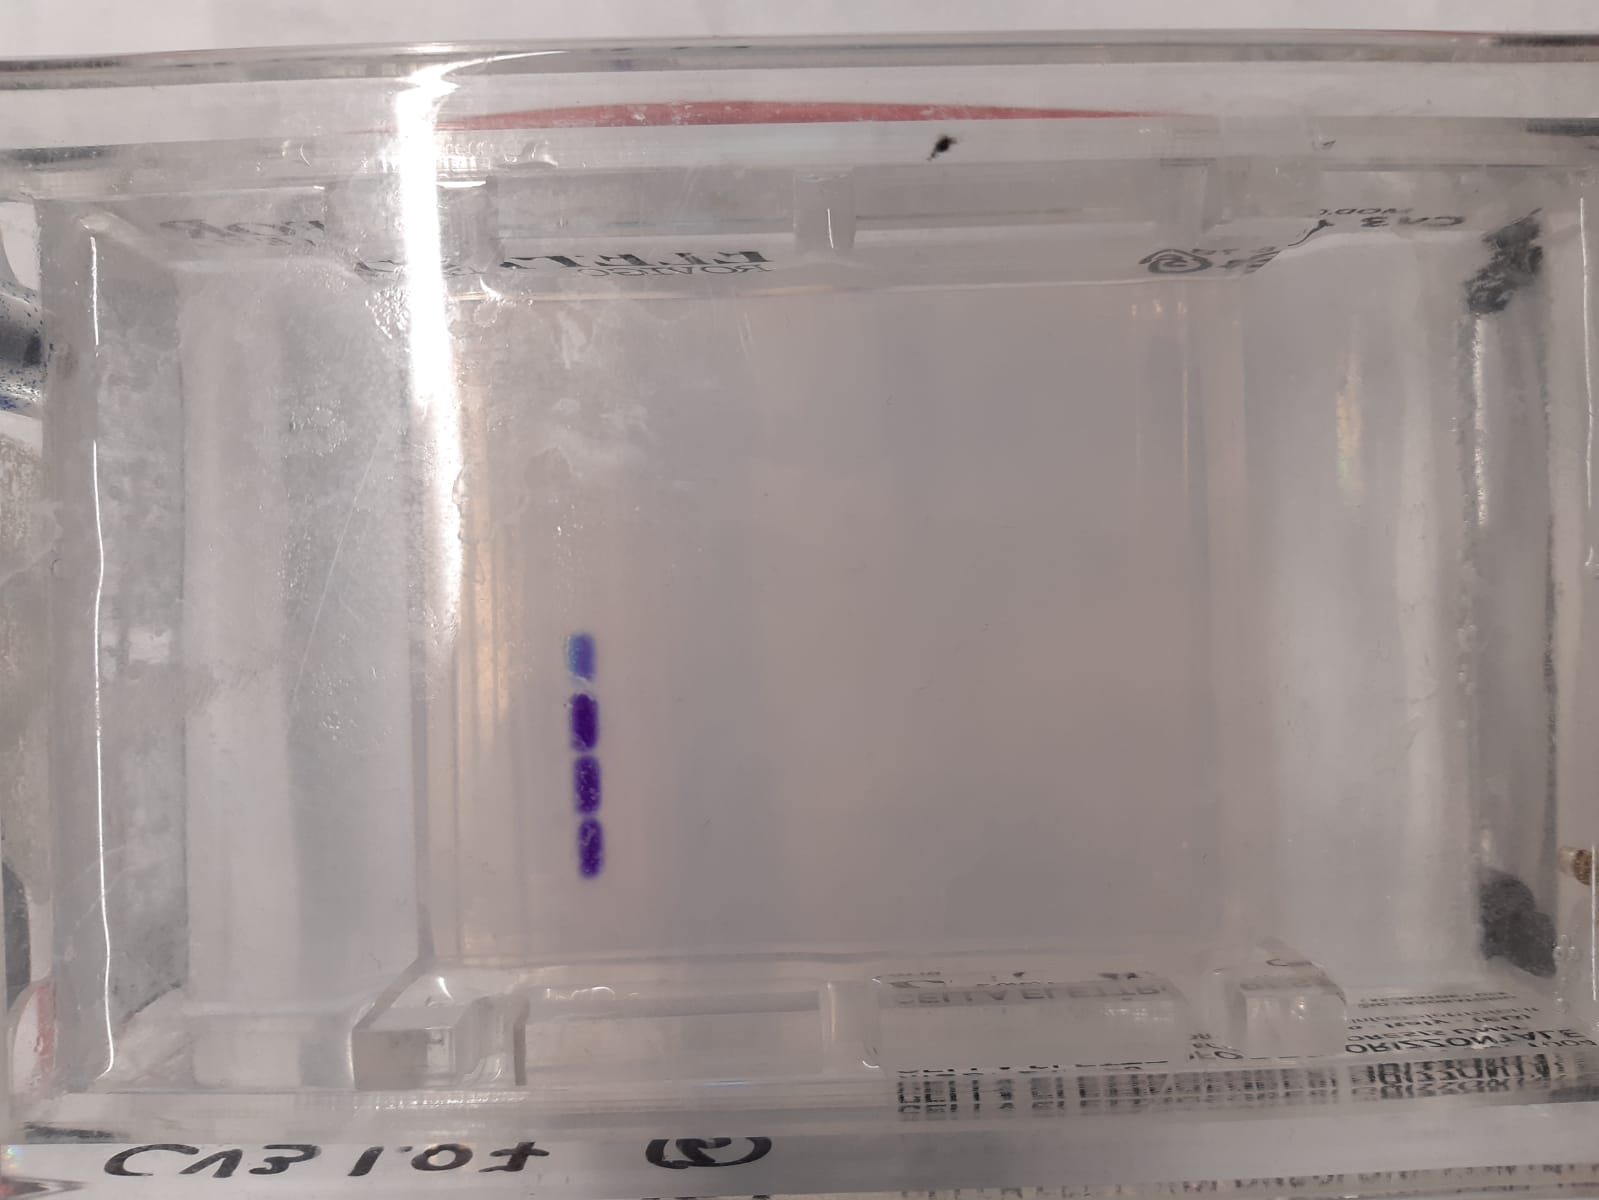
\includegraphics[
					width=4cm,
					height=6cm,
					trim={15cm 5cm 30cm 15cm},
					clip
					]{3-15}
				}
				\annotatedFigureText{0.63,0.325}{black}{1}{A}
				\annotatedFigureText{0.63,0.425}{black}{1}{B}
				\annotatedFigureText{0.63,0.525}{black}{1}{C}
				\annotatedFigureText{0.63,0.625}{black}{1}{D}
			\end{annotatedFigure}
			\caption[Piastra di agarosio]{\\Piastra di agarosio -
			\begin{enumerate}[person,label=\Alph*]
				\item DNA con enzima
				\item DNA senza enzima
				\item RNA
				\item Marker
			\end{enumerate}
			}
		\end{figure}
	}{}{}
\endgroup